\documentclass{article}
\usepackage[top=1in, bottom=1in, left=1in, right=1in]{geometry}
\usepackage{polski}
\usepackage[utf8]{inputenc}
\usepackage{multirow}
\usepackage{graphicx}
\usepackage{float}
\begin{document}
\title{\huge\bfseries Wyznaczanie ładunku właściwego elektronu metodą
poprzecznego pola magnetycznego (lampa Thomsona)}
\date{}
\author{}
\maketitle
\section{Wstęp teoretyczny}
\subsection{Elektron}
Elektron\footnote[1]{https://pl.wikipedia.org/wiki/Elektron, z dnia: 06.04.2017} jest to cząsteczka elementarna atomu o masie spoczynkowej równej
$$ m_e \approx 9,109\ 382\ 91 \cdot 10^{-31}\ kg$$
oraz o ładunku elektrycznym równym 
$$ e = -1,602\ 176\ 6208 \cdot 10^{-19}\ C$$
Ładunek właściwy elektronu wynosi
$$ \frac{e}{m_e} = -1,758\ 882\ 012 \cdot 10^{11}\ \frac{C}{kg}$$
\subsection{Ruch elektronu}
Siła Lorentza\footnote[2]{https://pl.wikipedia.org/wiki/Pole\_magnetyczne, z dnia: 06.04.2017} jest to siła jaka działa na cząstkę naelektryzowaną, wpadającą w pole magnetyczne o indukcji $\vec{B}$, z prędkością $\vec{v}$ wyrażana wzorem
$$\vec{F} = e(\vec{v} \times \vec{B})$$
Jeśli cząstka skierowana jest prostopadle do prędkości, wzór na siłę maksymalną przybiera formę
$$F_{max} = e \cdot v \cdot B$$
Prędkość $v$ elektronu rozpędzonego różnicą potencjałów $U$ określa wzór
$$v = \sqrt{\frac{2eU}{m}}$$
Gdy zostaje spełniony warunek kierunku prostopadłości do prędkości to tor ruchu staje się okręgiem o promieniu $r$. Siła Lorentza jest wtedy równa sile odśrodkowej działającej na elektron
$$F = e \cdot v \cdot B = \frac{mv^2}{r}$$
Po przekształceniu otrzymujemy 
$$v = \frac{ e \cdot B \cdot r}{m}$$
Wynika z tego, że ładunek właściwy elektronu możemy wyliczyć ze wzoru
$$\frac{e}{m} = \frac{2U}{B^2r^2}$$
\section{Przebieg i cel ćwiczenia}
Celem ćwiczenia jest wyznaczenie ładunku właściwego elektronu metodą poprzecznego pola magnetycznego, przy pomocy lampy Thomsona. Stanowisko pomiarowe składa się z lampy Thomsona, zasilacza lampy oraz zasilacza cewki Helmholtza, multimetra którego niepewność pomiarowa typu B wynosi
$$u(u) = \frac{1,5\% \cdot V + 5}{\sqrt{3}} = 3,75277675\ [V]$$
Pomiary rozpoczęliśmy od początkowej wartości napięcia równej $U = 300\ V$. Dla danego napięcia szukaliśmy takiego natężenia prądu $I$, aby uzyskać promienie wiązki elektronów równe $2$, $3$, $4$ i $5\ cm$. Następnie zmniejszaliśmy napięcie o $25\ v$. Badania zakończyliśmy dochodząc do $U = 100\ V$
\subsection{Opracowanie wyników}
Mierzone wyniki przedstawia tabela:
\begin{center}
\begin{tabular}{|c|c|c|c|c|}
\hline
\multirow{2}{*}{$U[V]$} & \multicolumn{4}{|c|}{$I_H[A]$}\\  
 & $r = 2\ cm$ & $r = 3\ cm$ & $r = 4\ cm$ & $r = 5\ cm$ \\ \hline  
$300$ & $3,81$ & $2,52$ & $1,95$ & $1,62$ \\ \hline 
$275$ & $3,5$ & $2,3$ & $1,85$ & $1,55$\\ \hline 
$250$ & $3,3$ & $2,2$ & $1,7$ & $1,5$\\ \hline 
$225$ & $2,97$ & $2,03$ & $1,61$ & $1,45$\\ \hline 
$200$ & $2,65$ & $1,75$ & $1,43$ & $-$\\ \hline 
$175$ & $2,4$ & $1,42$ & $-$ & $-$\\ \hline 
$150$ & $2,19$ & $1,19$ & $-$ & $-$\\\hline 
$125$ & $1,77$ & $-$ & $-$ & $-$\\ \hline 
$100$ & $1,4$ & $-$ & $-$ & $-$\\ \hline 
\end{tabular}
\end{center}
Aby przeliczyć wartość prądu cewek Helmholtza $I_H$ na wartość indukcji pola magnetycznego zastosowaliśmy wzór 
$$B = kI_H = \left(\frac{4}{5}\right)^{\frac{3}{2}} \mu \frac{N}{R} I_H$$
gdzie $\mu = 1,25664 \cdot 10^{-6}$ - bezwzględna  przenikalność  magnetyczna  próżni, $N = 124$ -  liczba  zwojów  w  cewkach Helmholtza, $R = 147.5\ mm$ – promień cewek.\\
Obliczone wyniki przedstawiliśmy w tabeli:
\begin{center}
\begin{tabular}{|c|c|c|c|c|}
\hline
\multirow{2}{*}{$U[V]$} & \multicolumn{4}{|c|}{$B$}\\  
 & $r = 2\ cm$ & $r = 3\ cm$ & $r = 4\ cm$ & $r = 5\ cm$ \\ \hline 
$300$ & $0,002880046$ & $0,001904913$ & $0,001474039$ & $0,001224587$\\ \hline 
$275$ & $0,002645712$ & $0,001738611$ & $0,001398448$ & $0,001171672$\\ \hline 
$250$ & $0,002494528$ & $0,001663019$ & $0,00128506$ & $0,001133877$\\ \hline 
$225$ & $0,002245076$ & $0,001534513$ & $0,001217027$ & $0,001096081$\\ \hline 
$200$ & $0,002003182$ & $0,001322856$ & $0,001080962$ & $-$\\ \hline 
$175$ & $0,001814202$ & $0,001073403$ & $-$ & $-$\\ \hline 
$150$ & $0,00165546$ & $0,000899542$ & $-$ & $-$\\ \hline 
$125$ & $0,001337974$ & $-$ & $-$ & $-$\\ \hline 
$100$ & $0,001058285$ & $-$ & $-$ & $-$\\ \hline 
\end{tabular}
\end{center}

Wiedząc, że zostaje spełniony warunek kierunku prostopadłości do prędkości możemy przyrównać wzór na siłę Lorentza oraz wzór na siłę odśrodkową działającą na elektron
$$F = e \cdot v \cdot B = \frac{mv^2}{r}$$
Po przekształceniu otrzymujemy 
$$v = \frac{ e \cdot B \cdot r}{m}$$
Co po kolejnym przekształceniu ukazuje nam zależność
$$ U = \frac{eB^2 r^2}{2m_e} $$
W kolejnym etapie opracowania wykreśliliśmy zależności $U(r^2 B^2)$ dla zadanych promieni(wartość $r^2B^2$ została pomnożona przez $10^{9}$ dla lepszej prezentacji wykresu):\\\\\
Zależność dla $r = 2cm$
\begin{figure}[H]
\centering
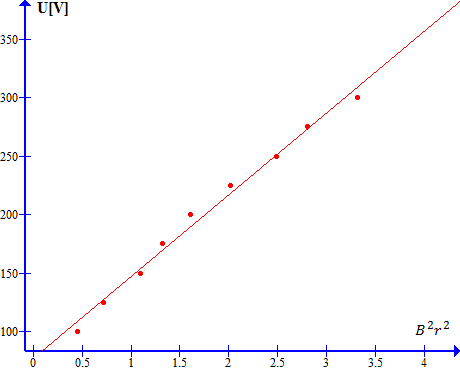
\includegraphics[width=13cm]{wykres1.png}
\end{figure}
Wzór na prostą przedstawia się wzorem
$$ f(x) = 69,9949x - 77,0819$$
Współczynnik kierunkowy prostej wynosił $a = 69,9949$ oraz współczynnik $b = -77,0819$.\\\\\\\\\\\\\\\\\\\\\\\\\\\\\\\\
Zależność dla $r = 3cm$
\begin{figure}[H]
\centering
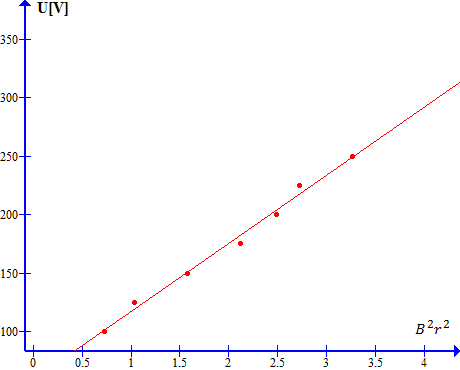
\includegraphics[width=15cm]{wykres2.png}
\end{figure}
Wzór na prostą przedstawia się wzorem
$$ f(x) = 58,3074x - 58,9281$$
Współczynnik kierunkowy prostej wynosił $a = 58,3074$ oraz współczynnik $b = -58,9281$.\\\\\\\\\\\\\\\\\\\\\\\\\\\\\\\\\\\\\\
Zależność dla $r = 4cm$
\begin{figure}[H]
\centering
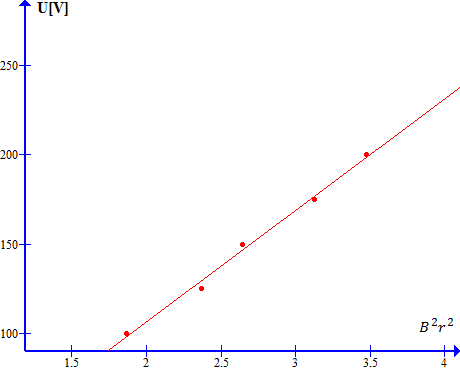
\includegraphics[width=15cm]{wykres3.png}
\end{figure}
Wzór na prostą przedstawia się wzorem
$$ f(x) = 62,5114x - 18,62$$
Współczynnik kierunkowy prostej wynosił $a = 62,5114$ oraz współczynnik $b = -18,62$.\\\\\\\\\\\\\\\\\\\\\\\\\\\\\\\\\\\\\\
Zależność dla $r = 5cm$
\begin{figure}[H]
\centering
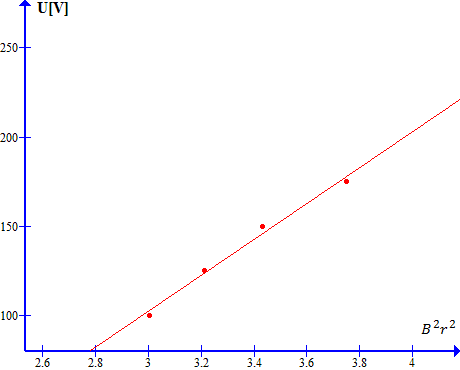
\includegraphics[width=15cm]{wykres4.png}
\end{figure}
Wzór na prostą przedstawia się wzorem
$$ f(x) = 61,7676x - 200,039$$
Współczynnik kierunkowy prostej wynosił $a = 61,7676$ oraz współczynnik $b = -200,039$.\\
Na podstawie wyznaczonych współczynników nachylenia wyznaczyliśmy ładunek właściwy $\frac{e}{m_e}$ dla danych promieni:
$$a = \frac{e}{2m_e}$$
\begin{center}
\begin{tabular}{|c|c|c|}
\hline
$r, m$ & $\frac{e}{m_e}, 10^9 [\frac{C}{kg}]$  \\ \hline 
$0,02$ & $139,9898$  \\ \hline 
$0,03$ & $116,6148$  \\ \hline 
$0,04$ & $125,0228$  \\ \hline 
$0,05$ & $123,5352$  \\ \hline 
\end{tabular}
\end{center}
Na podstawie prawa przenoszenia niepewności, obliczyliśmy niepewność wyznaczonej wartości ze wzoru 
$$u(\frac{e}{m_e}) = \sqrt{\Sigma[\frac{\delta y}{\delta x_k} \cdot u(x_k)]^2}$$
gdzie $x_k$ jest argumentem po którym obliczyliśmy pochodną.\\
$$u(\frac{e}{m_e}) = \sqrt{[\frac{2U}{2Br^2} \cdot u(B)]^2 + [\frac{2U}{2B^2r} \cdot u(r)]^2} \approx 3,93 \ [\frac{C}{kg}]$$ 


\begin{center}
\begin{tabular}{|c|c|c|}
\hline
$r, m$ & $u(\frac{e}{m_e}), 10^9 [\frac{C}{kg}]$  \\ \hline 
$0,02$ & $3,93$  \\ \hline 
$0,03$ & $6,33$  \\ \hline 
$0,04$ & $8,34$  \\ \hline 
$0,05$ & $5,86$  \\ \hline 
\end{tabular}
\end{center}
Za pomocą metody średniej ważonej uzyskaliśmy wynik
$$\frac{e}{m_e} = 126,29065 \cdot 10^9 [\frac{C}{kg}]$$
Niepewność rozszerzoną obliczyliśmy ze wzoru:
$$U(\frac{e}{m_e} )=k\cdot u(\frac{e}{m_e} ) = 12,23 \cdot 10^9 [\frac{C}{kg}]$$
gdzie k to współczynnik rozszerzenia równy $2$.\\
Więc uzyskany wynik to 
$$\frac{e}{m_e} = 126,29065 \cdot 10^9 \pm 12,23 \cdot 10^9 [\frac{C}{kg}]$$
Wartość tablicowa[1] obliczonej wartości wynosi
$$\frac{e}{m_e} = 175,8882012 \pm 0,00000015 \cdot 10^9 [\frac{C}{kg}]$$
\subsection{Wnioski}
Wartość obliczona i tablicowa znacznie nie zgadza się ze sobą. Może to być spowodowane niedoskonałością sprzętu pomiarowego oraz ludzkich zmysłów, gdyż badana wartość jest wartością opisującą cząsteczkę elementarną, więc nawet najmniejszy błąd pomiarowy skutkuje zupełnie innym wynikiem.
\begin{flushright}
\begin{scriptsize}
\textit{[1]http://const.physics.edu.pl/} \\
\end{scriptsize}
\end{flushright}
\end{document}